\documentclass[
	%a4paper, % Use A4 paper size
	letterpaper, % Use US letter paper size
]{jdf}

\addbibresource{references.bib}

\author{Nan Xiao}
\email{nanx@gatech.edu}
\title{CS6750 HCI Summer 2021:\\Assignment P4}

\begin{document}
%\lsstyle

\maketitle

\section{Question1 - Create GOMS model}
Objective: 
\begin{quote}
    Create a thorough GOMS model for contacting a professor to ask for an explanation of a grade.
\end{quote}

We will recap what is GOMS model from Joyner's lesson.

The GOMS Model (\cite{joyner2016a})
\begin{enumerate}
    \item G - Goals
    \item O - Operators
    \item M - Methods
    \item S - Selection rules
\end{enumerate}

Below is the GOMS model for the task.

\textbf{Initial Situation} - One have questions about a grade and need to contact a professor to ask for an explanation.
\begin{itemize}
    \item Selection rules - If the question is general and contains no sensitive information, one should choose to use a public post on the Edstem forum.
        \begin{itemize}
            \item \textbf{Methods - Edstem Public Post}
                \begin{itemize}
                    \item Operators - Enter URL of Edstem (30 secs)
                    \item Operators - Login with Gatech account username and password (30 secs)
                    \item Operators - Create new thread (3 secs)
                    \item Operators - Type in title (30 secs)
                    \item Operators - Select Category (30 secs)
                    \item Operators - Key in question (5 mins)
                    \item Operators - Leave Private unchecked (1 sec)
                    \item Operators - Click Post (1 sec)
                \end{itemize}
        \end{itemize}
    \item Selection rules - If the question is not a general one and contains personal information, one can choose to post privately on Edstem forum.
        \begin{itemize}
            \item \textbf{Methods - Edstem Private Post}
                \begin{itemize}
                    \item Operators - Enter URL of Edstem (30 secs)
                    \item Operators - Login with Gatech account username and password (30 secs)
                    \item Operators - Create new thread (3 secs)
                    \item Operators - Type in title (30 secs)
                    \item Operators - Select Category (30 secs)
                    \item Operators - Key in question (5 mins)
                    \item Operators - Check Private box (2 sec)
                    \item Operators - Click Post (1 sec)
                \end{itemize}
        \end{itemize}
    \item Selection rules - If there is someone asked related questions and get answered, you may be able to find the answer straight away. This should be used as the first method to try.
        \begin{itemize}
            \item \textbf{Methods - Search Edstem Post}
                \begin{itemize}
                    \item Operators - Enter URL of Edstem (30 secs)
                    \item Operators - Login with Gatech account username and password (30 secs)
                    \item Operators - Click Search box (1 sec)
                    \item Operators - Key in the question (1 min)
                    \item Operators - Find answer in search results (5 mins)
                \end{itemize}
        \end{itemize}
    \item Selection rules - If there is someone posted related questions but not exactly for your case, you may ask follow-up questions in that question thread.
        \begin{itemize}
            \item \textbf{Methods - Edstem Post follow-up question}
                \begin{itemize}
                    \item Operators - Enter URL of Edstem (30 secs)
                    \item Operators - Login with Gatech account username and password (30 secs)
                    \item Operators - Click Search box (1 sec)
                    \item Operators - Key in the question (1 min)
                    \item Operators - Find related question in search results (5 mins)
                    \item Operators - Click Add comment under that thread (1 sec)
                    \item Operators - Key in the follow-up question (5 mins)
                \end{itemize}
        \end{itemize}
    \item Selection rules - If you cannot find an answer on Edstem forum and not able to get reply using Edstem post, the last choice is to email the professor.
        \begin{itemize}
            \item \textbf{Methods - Email the professor}
                \begin{itemize}
                    \item Operators - Google Professor's name (10 secs)
                    \item Operators - Find Professor's website and click through (1 min)
                    \item Operators - Find Professor's email address on the website (3 min)
                    \item Operators - Open the email app (10 secs)
                    \item Operators - Copy Professor's email address to "Send-to" (10 secs)
                    \item Operators - Draft the email asking the question about the grade (5 mins)
                    \item Operators - Send out email (3 secs)
                \end{itemize}
        \end{itemize}
\end{itemize}
\textbf{Ultimate Goal} - You question about the grade is answered and you understand the explanation.

\section{Question2 - Create Hierarchical task analysis}
Objective: 
\begin{quote}
    Create a hierarchical task analysis of the task of submitting this assignment to Canvas and subsequently receiving one’s grade and feedback.
\end{quote}

While GOMS is using the processor view, Cognitive task analysis adopts the predictor view of a human's role in the system. It generally follows below common sequence: (\cite{joyner2016b})

\begin{enumerate}
	\item Collecting preliminary knowledge
	\item Identify knowledge representations
	\item Apply focused knowledge elicitation methods
	\item Analyze and verify data acquired
	\item Format results for the intended application
\end{enumerate}

Below is the Cognitive task analysis for the submitting assignment and getting feedback task.

\textbf{Top level task} - Submitting this assignment to Canvas and subsequently receiving one’s grade and feedback
\begin{itemize}
    \item \textbf{Sub-task} - Submitting this assignment to Canvas
        \begin{itemize}
            \item Sub-sub-task - Find Canvas assignment page
                \begin{itemize}
                    \item Operator - Entering a Canvas URL
                    \item Operator - Clicking Course page
                    \item Operator - Clicking Assignments page
                    \item Operator - Scrolling down to the correct assignment
                    \item Operator - Clicking that assignment link
                \end{itemize}
            \item Sub-sub-task - Upload assignment in the assignment page
                \begin{itemize}
                    \item Operator - Clicking Start Assignment button
                    \item Operator - Selecting a file from the file browser
                    \item Operator - Selecting Choose a file
                    \item Operator - Selecting the correct file and click Open
                \end{itemize}
            \item Sub-sub-task - Add more assignment files in the assignment page
                \begin{itemize}
                    \item Operator - Clicking Add another file button
                    \item Operator - Selecting a file from the file browser
                    \item Operator - Selecting Choose a file
                    \item Operator - Selecting the correct file and click Open
                \end{itemize}
            \item Sub-sub-task - Submit assignment
                \begin{itemize}
                    \item Operator - Selecting "Agree to the agreement"
                    \item Operator - Clicking Submit Assignment button
                \end{itemize}
            \end{itemize}
    \item \textbf{Sub-task} - Receiving one’s grade and feedback
        \begin{itemize}
            \item Sub-sub-task - Find Canvas Assignments page
                \begin{itemize}
                    \item Operator - Entering a Canvas URL
                    \item Operator - Clicking Course page
                    \item Operator - Clicking Assignments page 
                \end{itemize}
            \item Sub-sub-task - Find grade on the Assignments page
                \begin{itemize}
                    \item Operator - Scrolling down to the correct assignment
                    \item Operator - Reading the score under assignment name
                \end{itemize}
            \item Sub-sub-task - Find the assignment sub-page that specific to the target assignment
                \begin{itemize}
                    \item Operator - Clicking the target assignment
                \end{itemize}
            \item Sub-sub-task - Find the feedback on the assignment sub-page
                \begin{itemize}
                    \item Operator - Reading the feedback on the right side of page
                    \item Operator - Scrolling down to read the full feedback
                \end{itemize}
        \end{itemize}
\end{itemize}


\section{Question3 - The system for navigation}

According to Joyner (\cite{joyner2016b})
\begin{quotation}
    \noindent “Distributed Cognition suggests models of cognition should be extended outside the mind."
\end{quotation}
In this section, we will analyze the distributed cognition for navigation tasks.

\subsection{The system for navigation comprised a married couple, a map, and street name sign}

We can summarize how the cognitive activities are distributed in the system in Table 1 below.

\begin{table}[h] % [h] forces the table to be output where it is defined in the code (it suppresses floating)
	\caption{Navigation for a couple driving with a map}
	\small % Reduce font size
	\centering % Centre the table
	\begin{tabular}{L{0.2\linewidth} L{0.2\linewidth} L{0.4\linewidth}}
		\textbf{Cognition} & \textbf{Component} & \textbf{Cognitive Activity}\\
		\toprule[0.5pt]
		Long-Term Memory & Map & Where the car has gone through so far \\
		\midrule
		Long-Term Memory & Map & What is the route to the destination \\
		\midrule
		Short-Term Memory & Street name sign & Where is the car currently at \\
		\midrule
		Short-Term Memory & Street name sign & When to turn left/right if you want to go certain places on the map \\
		\midrule
		Short-Term Memory & Passenger & Where is the car currently at on the map \\
		\midrule
		Working Memory & Passenger & What to do in the next crossing \\
		\midrule
		Working Memory & Driver & What is the traffic now \\
		\midrule
		Deliberation & Driver & Whether to turn left, right or keep straight \\
	\end{tabular}
\end{table}


\subsection{Compare and contrast this same situation with a lone driver using a GPS}
Without a passenger, the below tasks will be replaced with GPS as shown in table 2 below.

\begin{table}[h] % [h] forces the table to be output where it is defined in the code (it suppresses floating)
	\caption{GPS vs Passenger in handling navigation cognitive tasks}
	\small % Reduce font size
	\centering % Centre the table
	\begin{tabular}{L{0.4\linewidth} L{0.2\linewidth} L{0.4\linewidth}}
		\textbf{Cognitive Activities} & \textbf{GPS} & \textbf{Passenger}\\
		\toprule[0.5pt]
		Understand overall route planning & Show in GPS map & Read the map \\
		\midrule
		Understand when to turn left or right & Use GPS with map and voice instructions & Use physical map and road signs to figure out \\
		\midrule
		Understand where the car current is & Use GPS with map to show & Estimation based on map and surroundings \\
		\midrule
		Notice traffic around & Missing & Through observation \\
		\midrule
		Rephrase instruction if driver do not understand & Missing & Through conversation \\
		\midrule
		Suggest change of route & Missing & Based on conversation to change the plan\\
		\midrule
		Suggest to take a rest & Missing & Through observation that drive is tired \\
	\end{tabular}
\end{table}

\subsection{What does social cognition reveal about the situation that distributed cognition does not}

From table 2 we can see that, GPS can do a good job if we use it to map the distributed cognition. It can give instructions to the driver when to turn and show the overall plan to the destination, just like a passenger will do. And it may do better at this because of the visual interface. But through social cognition analysis, we can see that several social components are missing by using GPS instead of having a human aside. The GPS cannot help drive to notice the traffic around, rephrase instructions if seeing driver confused, or make a suggestion to change the route or take a rest. If it is a long journey, having a conversation with the passenger will also reduce the tiredness of the driver.

\subsection{How might the social relationships among the parts of the system affect the success of the system as a whole}

Social relationships among the parts of the system can help to reduce the cognitive load of the individual parts, and many activities that can be distributed using social relationships cannot be replaced by artefacts yet as shown in the previous table 2. In this way, social relationships reduce cognitive effort and individuals can have more working memory to accomplish the tasks. The system as a whole has a higher chance of success.


\section{Question4 - Task analysis from the perspective of distributed cognition}

\subsection{Identity and briefly describe the task you’ve chosen and the interface associated with it}
The task chosen here is collaboratively writing documentation on Google doc. Currently, a lot of group projects or products need a team to write together on an online platform. Google doc is one of the best options. The main interface of Google Docs is like a simplified version of what we already have in Microsoft Word as shown in Figure 1. Collaborative works are shown in the interface.

\begin{figure}[h]
	\centering
	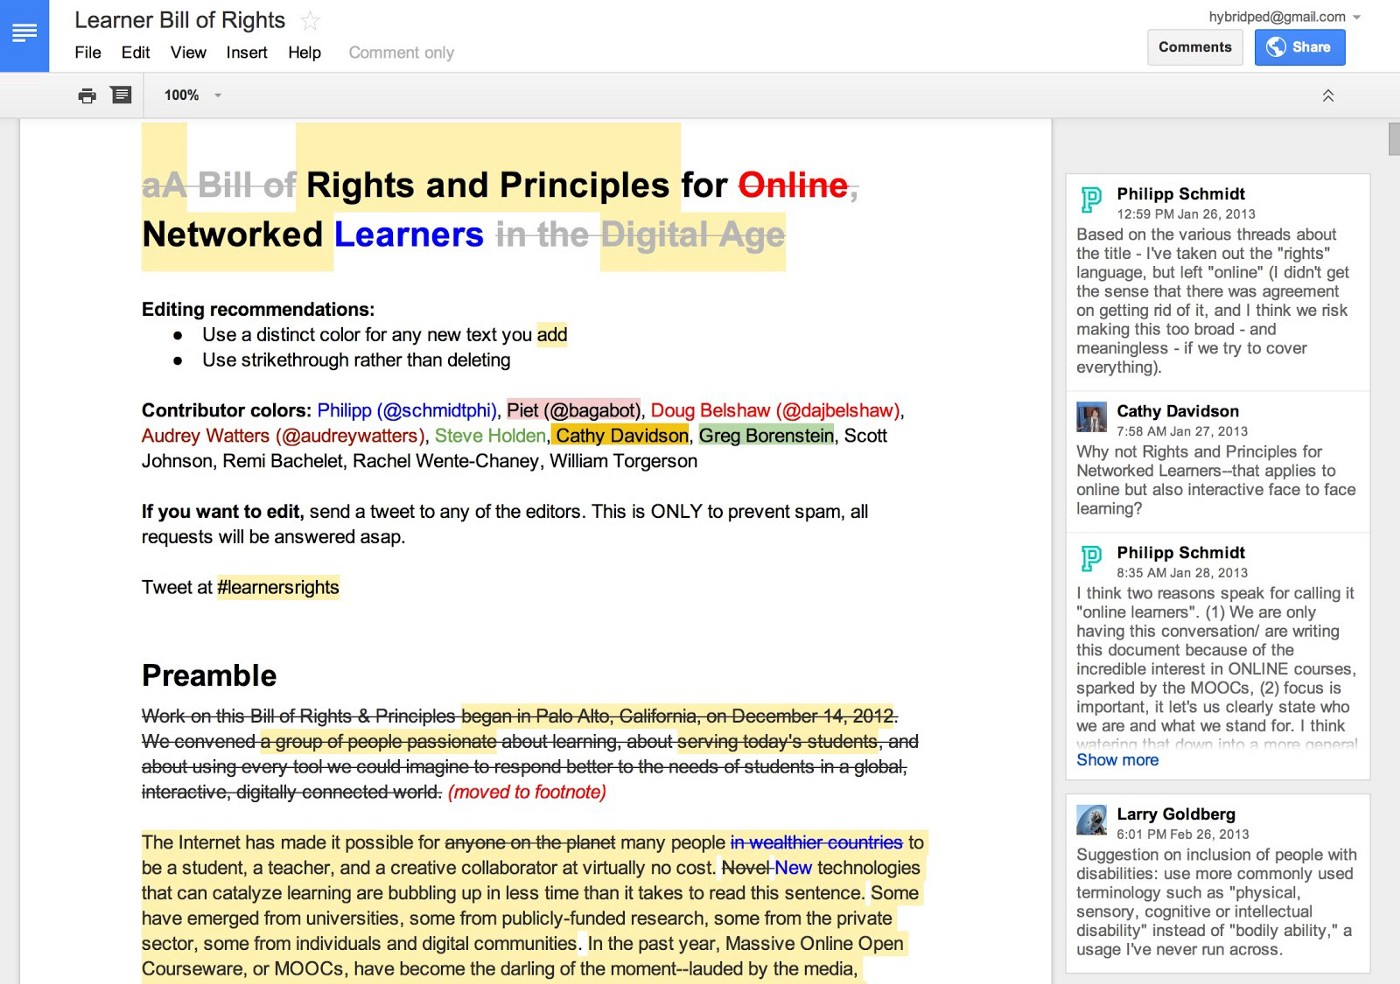
\includegraphics[height=6cm]{jdf-latex/Figures/google_doc.jpeg}
	\caption{Main interface - Collaborating on Google Doc}
	\label{fig:googledoc}
\end{figure}


\subsection{Describe the pieces of the system}

The interface has a big "Share" button to let you control who you want to share the document with. It has a version history of how files changed through the timeline and shows when and who changed which content. One can use the editor tools to alter the size and font of the text or change the alignment and indent. Also, one can highlight part of the content and add comments. On the top of the interface, there is a status indicating who is currently on this page. In the main content, there are cursors in different colours indicating who is currently writing on which part of the document.

\subsection{Describe what cognitive tasks are performed by each member of the system, both human and artefact alike}

\begin{table}[h] % [h] forces the table to be output where it is defined in the code (it suppresses floating)
	\caption{Cognitive tasks by each member of the system}
	\small % Reduce font size
	\centering % Centre the table
	\begin{tabular}{L{0.2\linewidth} L{0.2\linewidth} L{0.4\linewidth}}
		\textbf{Member} & \textbf{Task Category} & \textbf{Cognitive Task}\\
		\toprule[0.5pt]
		Human & Reasoning and action & Writing the content \\
		\midrule
		Cursor & Perception & Understand where one is writing, and where the others are writing now \\
		\midrule
		History versions & Memory & Remember what is the historical versions of the content \\
		\midrule
		Highlighting and comments & Memory & Save other people's feedback \\
		\midrule
		Editor tools & Perception and action & Alter the content formatting, the icons reduce the cognitive effort \\
		\midrule
		User status & Perception & Understand who is currently active on this document \\
		\midrule
		Auto suggestion & Action & Help to avoid misspelling \\
	\end{tabular}
\end{table}

Cognitive tasks performed by each member of the system are summarized in table 3. 

\section{References}
\printbibliography[heading=none]


\end{document}